\documentclass[11pt,a4paper]{article}
\usepackage[T1]{fontenc}
\usepackage{lmodern,microtype,amsmath,amssymb,amsthm,booktabs}
\usepackage{tikz}
\usepackage[margin=25mm,top=23mm,bottom=23mm]{geometry}
\usepackage{xcolor}
\usepackage[hidelinks]{hyperref}
\pagestyle{empty}
\setlength{\parindent}{0pt}
\setlength{\parskip}{5pt plus 1pt minus 1pt}
\setlength{\abovedisplayskip}{7pt plus 2pt minus 2pt}
\setlength{\belowdisplayskip}{7pt plus 2pt minus 2pt}
\setlength{\emergencystretch}{1.3em}
\newtheorem{theorem}{Theorem}
\newtheorem{lemma}[theorem]{Lemma}
\newtheorem{corollary}[theorem]{Corollary}
\newcommand{\F}{\mathcal F}
\newcommand{\NN}{N}
\newcommand{\smalltitle}[1]{\par\medskip\noindent\textbf{#1}\enspace}
\hypersetup{pdfauthor={Haimin Zhou},pdfkeywords={triangle packing, triangle transversal, Tuza conjecture, book size}}
\begin{document}

{\small\scshape Research manuscript \hfill 20 November 2026}
\medskip

{\LARGE\bfseries A uniform gap below two for triangle packings\\[-1pt]
and edge transversals in \(K_4\)-free graphs\\[-1pt]
of book size at most three\par}
\medskip

{\large Haimin Zhou\par}
{\small Independent Researcher \quad
\href{mailto:haiminzhou.1@gmail.com}{haiminzhou.1@gmail.com}\par}
{\small Version 1.0.1: attribution and archival revision\par}
\medskip

Let \(\nu_\triangle(G)\) be the largest number of edge-disjoint triangles of
a finite simple graph \(G\), and let \(\tau_\triangle(G)\) be the least
number of edges meeting every triangle. Write \(b(G)\) for the maximum
number of triangles containing one edge, taking zero for an edgeless graph.

\begin{theorem}\label{thm:main}
If \(G\) is \(K_4\)-free and \(b(G)\le3\), then
\[
              177\,\tau_\triangle(G)\ \le\ 353\,\nu_\triangle(G).
\]
The same bound holds for covering and packing any specified family
\(\F\) of triangles of \(G\).
\end{theorem}

The upper bound has no density or connectivity hypothesis. For \(b(G)\le2\)
in the \(K_4\)-free class, Haxell, Kostochka and Thomassé
proved the sharp bound \(3/2\) \cite{hktflat}. Their \(K_4\)-free examples
with ratio approaching two have unbounded book size \cite{hktfrac}.
For \(b(G)\le3\), Munaro's Theorem 9 gives \(193/98\) when every triangle
shares an edge with at most four other triangles \cite{munaro}.
The present bound includes conflict degrees five and six and their mixtures.
Tsujimura's recent theorem allows certain four-page edges and uses a maximum
average degree bound that can be placed on an induced core \cite{tsu}.

\section*{1. The graph of triangle intersections}

Fix \(\F\), possibly empty. Its \emph{conflict graph} \(H\) has the triangles
of \(\F\) as vertices and adjacency for a shared graph edge. Write \(n=|\F|\)
and \(a=\alpha(H)\). A \emph{book} at an edge consists of the triangles of
\(\F\) containing that edge. The number of its triangles is its size. Three
pairwise adjacent triangles without a common edge would form three faces of
a \(K_4\). Consequently every clique of \(H\) lies in a book. Indeed, two
distinct triangles determine their common edge uniquely, and every further
triangle in their clique must use it. A singleton can be assigned any side.
Thus \(\theta(H)\), the minimum number of cliques covering \(V(H)\), is the
edge transversal number of \(\F\), and \(a\) is its packing number.

For \(w\in V(H)\) let \(P(w)\) be its three book sizes in decreasing order,
written as a three-digit string. Its degree is \(d_w=\sum_{k\in P(w)}(k-1)\),
where entries are counted with multiplicity. Throughout, deleting triangles
means passing to the induced conflict graph and recomputing the book sizes
within the surviving family. A surviving family need not comprise all
triangles in the union of its edges.

The proof combines a packing weight for each of the ten profiles with a
random edge cover. A matching among faces with one single-page side improves
that cover. Its unmatched faces seed a packing in which locally improving
moves leave an explicitly bounded degree deficit.

\newpage
\section*{2. An additive packing bound}

The following table defines integer weights \(F(P)\). Write \(g_k(P)\)
for the increment in \(F\) when one entry \(k\) is reduced to \(k-1\),
for \(k=2,3\) present in \(P\). Blank entries are inapplicable. Define
\[
 L(P)=(d+1)F(P)-
     \sum_{\substack{k\in P\\ k\ge2}}(k-1)(d+1-k)g_k(P).
\]
The final column will be used in Section 3.

\begin{center}
\begin{tabular}{crrrrrr}
\toprule
\(P\)&\(d\)&\(F(P)\)&\(g_2(P)\)&\(g_3(P)\)&\(L(P)\)&\(768c(P)\)\\
\midrule
111&0&780& & &780&768\\
211&1&390&390& &780&624\\
221&2&312&78& &780&528\\
311&2&260& &130&780&544\\
222&3&265&47& &778&456\\
321&3&239&21&73&768&472\\
322&4&218&21&47&776&412\\
331&4&207& &32&779&428\\
332&5&192&15&26&780&374\\
333&6&173& &19&755&339\\
\bottomrule
\end{tabular}
\end{center}

\begin{lemma}\label{lem:pot}
\(\displaystyle W(H):=\sum_{w\in V(H)}F(P(w))\le780\,\alpha(H).\)
\end{lemma}
\begin{proof}
For a fixed \(k\), the table gives nonnegative increments, and
\(g_k(P)\ge g_k(Q)\) whenever \(d(P)<d(Q)\) and both values exist.
Delete a closed neighborhood \(\NN[v]\). A surviving face \(w\) loses
at most one other page on any one of its sides. Indeed, for two such
lost pages \(u,u'\) on that side, either \(v\in\{u,u'\}\), which would
delete \(w\), or \(v,u,u'\) are pairwise adjacent and hence lie in
the same book, which also deletes \(w\). As several distinct sides
decrease, take their decrements in any order. Each untouched side still
has its original size, while \(d\) has dropped. The total gain in \(F(P(w))\)
is therefore at least the sum of its initial increments for the lost pages.

Sum the loss \(W(H)-W(H-\NN[v])\) over all choices of \(v\).
Each \(w\) contributes \((d_w+1)F(P(w))\) in deletions. For \(u\sim w\)
in a book of size \(k\), \(\NN[u]\cap\NN[w]\) is exactly this book.
There are \(d_u+1-k\) choices of \(v\) that delete \(u\) and retain \(w\).
The surviving gains on the two directions of \(uw\) are bounded below by
\((d_u+1-k)g_k(P(w))+(d_w+1-k)g_k(P(u))\).
Subtracting the expression with each increment aligned to its own degree
gives \((d_u-d_w)(g_k(P(w))-g_k(P(u)))\ge0\). Thus the summed loss
is at most \(\sum_w L(P(w))\le780n\). If \(n>0\), some deletion loses
at most 780. A packing of the remainder extends by \(v\).
Induction, beginning with the empty family, proves the assertion.
\end{proof}

\newpage
\section*{3. A random edge cover and its matching saving}

Color the vertices of \(G\) independently with two equally likely colors.
For each triangle having both colors, take its unique monochromatic side.
After taking the union of these sides, add one edge for each triangle still
uncovered. An edge of a size-\(k\) book is taken initially with probability
\(\frac12-2^{-(k+1)}\). Indeed its endpoints must agree and at least one
of the \(k\) other vertices must have opposite color. A specified face
is uncovered initially exactly when all three of its vertices and all its
external page tips on its sides have one color. Each external tip occurs on
just one side, since a vertex adjacent to the three face vertices makes
a \(K_4\). Thus there are \(d\) distinct external tips. Assign the expected
cost of an initially selected edge equally to its pages. The expected total
cover size is at most \(\sum_w c(P(w))\), where
\begin{equation}\label{eq:color}
c(P)=2^{-(d+2)}+\sum_{k\in P}\frac{1/2-2^{-(k+1)}}{k}.
\end{equation}

\begin{corollary}\label{cor:two}
Every specified family satisfies \(\theta(H)\le 2\alpha(H)\).
\end{corollary}
\begin{proof}
The empty family is immediate.
If every used edge has at least two pages and the family is nonempty, the
four table rows \(222,322,332,333\) give \(c(P)<2F(P)/780\).
Hence the inequality is strict by Lemma~\ref{lem:pot}.
Otherwise take a face \(v\) having a single-page side. The other two
sides cover \(\NN[v]\). A packing of \(H-\NN[v]\) extends by \(v\).
Induction on \(|\F|\), including the empty base case, proves the claim.
\end{proof}

Let \(S\) be the set of faces having \emph{exactly one} single-page side
and \(s=|S|\). Fix a maximum matching \(M\) in \(H[S]\) of size \(\mu\).
The set \(U=S\setminus V(M)\) is independent and \(t=|U|=s-2\mu\).

\begin{lemma}\label{lem:matched}
\(\displaystyle \theta(H)\le\sum_w c(P(w))-\mu/8.\)
\end{lemma}
\begin{proof}
A matched pair has a common side \(xy\) and distinct third vertices \(z,w\).
With probability \(1/2\) the colors of \(x,y\) differ. Given their colors,
each of \(z,w\) has exactly one choice making its face's single-page side
the unique monochromatic side. These two choices are independent, giving
probability \(1/8\) overall. On that event the initial cover contains the
two single-page sides. Replace them by \(xy\), saving at least one edge.
Each deleted side covers only its own face. The matched pairs are
vertex-disjoint in \(H\), so the deleted sides are all distinct, and an
inserted common side cannot itself be a deleted single-page side. All the
exchanges can be made simultaneously, preserving coverage and any
supplemental edges still needed. Linearity of expectation gives the bound.
\end{proof}

\newpage
\section*{4. A cover from a locally optimal packing}

Call an independent set \(I\) locally optimal if no larger independent
set is obtained by deleting at most two members of \(I\) and adding new
vertices. In particular \(I\) is maximal. Set \(p=|I|\) and
\(D(I)=\sum_{i\in I}(6-d_i)\).

\begin{lemma}\label{lem:local}
Every such \(I\) satisfies \(\theta(H)\le 11p-2n-D(I)\).
\end{lemma}
\begin{proof}
Call members of \(I\) roots. Every outside face sees one to three roots,
since each of its sides is shared with at most one root. Let \(r_j\)
count the faces seeing \(j\) roots. At root \(i\), its private faces
\(P_i\) see only \(i\). They form a clique by the one-for-two exchange,
so \(|P_i|\le2\). If nonempty, they share one side \(c_i\) with \(i\).
Let \(a_j\) count the roots with \(j\) private faces. We have
\(r_1=a_1+2a_2\) and \(\sum_i d_i=r_1+2r_2+3r_3\).
As \(n=p+r_1+r_2+r_3\), these give
\begin{equation}\label{eq:count}
2n=9p+a_2-a_0-r_3-D(I).
\end{equation}

Select the three sides of each root with no private faces and \(c_i\)
at each remaining root. This covers every root and every one-root face.
Both roots of an uncovered two-root face have nonempty private sets.
An uncovered face \(b\) seeing just two roots
\(i,j\) cannot be adjacent to any member of \(P_i\) or \(P_j\), since a
clique with that root would force \(b\) to use its selected side.
The bipartite adjacencies between \(P_i\) and \(P_j\) form a matching.
Indeed a face meeting two privates of the other root must be in their
common book and hence meet that other root. If either set has size two,
some cross-pair is nonadjacent and its two faces together with \(b\)
replace \(i,j\). If both are singletons \(q_i,q_j\), the same exchange
requires \(q_i\sim q_j\). Thus every remaining two-root face gives an
induced five-cycle \(i,q_i,q_j,j,b\).

By Munaro's five-wheel lemma \cite[Lemma 9]{munaro}, these five triangles
are the consecutive faces of a wheel with a common center. Inducedness
persists in the full triangle graph because adjacency among the five faces
is unchanged. At a single-private root \(i=uva\) with private \(q_i=uvz\),
label its free side \(ua\) by \(uz\) and \(va\) by \(vz\). By the wheel
description, the two free sides used by \(b\) have the same label, the
side of \(q_i\) shared with \(q_j\). In fact if the center is \(u\), the
shared root side is \(ua\) and the label is \(uz\); exchanging \(u,v\)
gives the other case.

Form a graph on the \(2a_1\) free sides by joining the two sides of each
remaining two-root face. Each label occurs on at most three positions,
since the corresponding private triangles are distinct members of its
book. A free side meets exactly one endpoint of its label. A constraint
for label \(uv\) joins two positions incident to the same endpoint, the
wheel center. Three pairwise constrained positions would
therefore have a common center \(u\), say \(ux,uy,uz\) with distinct ends
(roots are edge-disjoint). The corresponding constraints force \(xy,yz,zx\),
giving a \(K_4\). Hence each label induces a triangle-free simple graph of
order at most three, with a vertex cover of size at most half its order.
At most \(a_1\) free sides consequently suffice. Add one side for each still
uncovered three-root face. The cost is at most
\(3a_0+2a_1+a_2+r_3=2p+a_0-a_2+r_3\). Equation~\eqref{eq:count}
gives the lemma.
\end{proof}

\begin{center}
\begin{minipage}{.34\linewidth}\centering
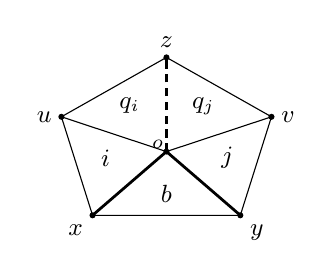
\begin{tikzpicture}[scale=.92, every node/.style={font=\small}]
  \coordinate (o) at (0,0);
  \coordinate (x) at (-1.02,-.88);
  \coordinate (u) at (-1.45,.48);
  \coordinate (z) at (0,1.30);
  \coordinate (v) at (1.45,.48);
  \coordinate (y) at (1.02,-.88);
  \draw[thin] (x)--(u)--(z)--(v)--(y)--cycle (u)--(o)--(v);
  \draw[line width=1.0pt] (x)--(o)--(y);
  \draw[densely dashed,line width=.8pt] (o)--(z);
  \foreach \p in {o,x,u,z,v,y} \fill (\p) circle (1.2pt);
  \node[below left] at (x) {\(x\)};
  \node[left] at (u) {\(u\)};
  \node[above] at (z) {\(z\)};
  \node[right] at (v) {\(v\)};
  \node[below right] at (y) {\(y\)};
  \node[above left,inner sep=1pt] at (o) {\scriptsize \(o\)};
  \node at (-.84,-.09) {\(i\)};
  \node at (-.51,.63) {\(q_i\)};
  \node at (.51,.63) {\(q_j\)};
  \node at (.84,-.09) {\(j\)};
  \node at (0,-.58) {\(b\)};
\end{tikzpicture}
\end{minipage}\hspace{1em}%
\begin{minipage}{.54\linewidth}\small
The five-wheel in Lemma~\ref{lem:local}. The free sides \(ox\) and \(oy\)
of the roots \(i\) and \(j\) both carry the label \(oz\), shared by the
private faces \(q_i,q_j\). Selecting either free side covers \(b\).
\end{minipage}
\end{center}

\newpage
\section*{5. Retaining unmatched faces and closing the gap}

Write \(e=2a-\theta(H)\). Corollary~\ref{cor:two} gives \(e\ge0\)
in every subfamily before the following use of the deficit.

\begin{lemma}\label{lem:retain}
For \(S,M\) as in Section 3,
\(\displaystyle 2n+2s-4\mu\le9a+3e.\)
\end{lemma}
\begin{proof}
The closed neighborhood of \(U\) is covered using at most \(2t\) edges.
For \(R=H-\NN[U]\), Corollary~\ref{cor:two} gives
\(\theta(H)\le2t+2\alpha(R)\). Consequently \(U\) together with a maximum
packing of \(R\) has size \(t+\alpha(R)\ge a-e/2\). Starting there,
perform strictly improving moves deleting at most two current roots until
there are no such moves. At most \(e/2\) moves occur, since each increases
cardinality by at least one. The final locally optimal packing \(I\) retains
at least \(t-e\) of the original unmatched faces. Each of them has degree
at most four in \(H\), so \(D(I)\ge 2(t-e)\), also when \(t-e<0\).
Lemma~\ref{lem:local} and \(|I|\le a\) now give
\(2a-e\le11a-2n-2(t-e)\). Substitute \(t=s-2\mu\).
\end{proof}

\begin{proof}[Proof of Theorem~\ref{thm:main}]
Use induction on \(n\). If a face \(v\) has at least two single-page sides,
one side covers \(\NN[v]\) and \(a\ge1+\alpha(H-\NN[v])\).
The inductive inequality on the remainder therefore extends, since
\(353/177>1\). The empty family satisfies the assertion. In every
other case the seven remaining rows obey
\begin{equation}\label{eq:price}
 c(P)\le\frac{11}{6}\frac{F(P)}{780}
           +\frac{1+\boldsymbol{1}_{\{P\ \mathrm{has\ a\ single\ page}\}}}{28}.
\end{equation}
In the order \(221,222,321,322,331,332,333\) the right side minus the
left, with common denominator \(1\,048\,320\), has numerators
\[
122928,\quad67960,\quad19496,\quad12212,\quad708,\quad18,\quad977.
\]
Summing \eqref{eq:price}, using Lemmas~\ref{lem:pot}, \ref{lem:matched},
and \ref{lem:retain}, and \(1/8\ge4/56\), gives
\begin{align*}
 \theta(H)
 &\le \frac{11}{6}a+\frac{n+s}{28}-\frac{\mu}{8}\\
 &\le \frac{11}{6}a+\frac{2n+2s-4\mu}{56}
 \le \frac{335}{168}a+\frac{3}{56}e .
\end{align*}
As \(\theta(H)=2a-e\), it follows that \(a/168\le59e/56\).
Thus \(a\le177e\), proving \(177\theta(H)\le353a\).
\end{proof}

The five-wheel \(K_1\vee C_5\) has packing number two and edge transversal
number three. Every edge meets at most two of its five triangles, and three
suitably chosen spokes cover them. Its conflict graph is \(C_5\).
Thus the optimal coefficient throughout this class lies in
\([3/2,353/177]\).

\newpage
\renewcommand{\refname}{Sources and verification}
\begin{thebibliography}{9}
\bibitem{br} A. Bo\ss ecker and D. Rautenbach,
Interpolating between bounds on the independence number,
\emph{Discrete Mathematics} 310 (2010), 2398--2403.
\href{https://doi.org/10.1016/j.disc.2010.05.026}{doi:10.1016/j.disc.2010.05.026}.

\bibitem{hktfrac} P. Haxell, A. Kostochka and S. Thomassé,
A stability theorem on fractional covering of triangles by edges,
\emph{European Journal of Combinatorics} 33 (2012), 799--806.
\href{https://perso.ens-lyon.fr/stephan.thomasse/liste/fractuza.pdf}{Authors' manuscript}.

\bibitem{hktflat} P. Haxell, A. Kostochka and S. Thomassé,
Packing and covering triangles in \(K_4\)-free planar graphs,
\emph{Graphs and Combinatorics} 28 (2012), 653--662.
\href{https://perso.ens-lyon.fr/stephan.thomasse/liste/packplanar.pdf}{Authors' manuscript}.

\bibitem{munaro} A. Munaro, Triangle packings and transversals of some
\(K_4\)-free graphs, \emph{Graphs and Combinatorics} 34 (2018), 647--668.
\href{https://doi.org/10.1007/s00373-018-1903-y}{doi:10.1007/s00373-018-1903-y}.

\bibitem{shearer} J. B. Shearer, A note on the independence number of
triangle-free graphs, II, \emph{Journal of Combinatorial Theory, Series B}
53 (1991), 300--307.
\href{https://doi.org/10.1016/0095-8956(91)90080-4}{doi:10.1016/0095-8956(91)90080-4}.

\bibitem{tsu} Y. Tsujimura, Triangle-overlap cores and density bounds for
Tuza's conjecture, 2026.
\href{https://arxiv.org/html/2611.11128v2}{arXiv:2611.11128v2}.
\end{thebibliography}

\smalltitle{Relation to previous methods.}
The averaging over closed neighborhoods in Lemma~\ref{lem:pot} follows
the approach of Shearer \cite{shearer} and its extension to graphs with local triangles
by Bo\ss ecker and Rautenbach \cite{br}. Here the weight and its two
increments depend on the individual book sizes. Munaro's wheel lemma is
used in Lemma~\ref{lem:local}. The resulting count applies to a packing
locally optimal under the deletion of at most two members. This distinction
allows the retention argument in Lemma~\ref{lem:retain}.

\smalltitle{Scope.}
The density hypothesis in \cite{tsu} uses maximum average degree, the
maximum of \(2|E(J)|/|V(J)|\) over nonempty subgraphs \(J\). Its localization
includes all original edges between vertices in the core. Theorem~\ref{thm:main}
allows arbitrary densities and adds \(K_4\)-freeness and a book bound of three.
For the broader class permitting the specified four-page edges, eliminating
the density hypothesis remains a separate problem.

\smalltitle{Verification.}
All numerical premises for the infinite theorem are the ten integer rows
in Section 2 and the seven differences in Section 5. They can be checked by
substitution. The accompanying research record includes two independent
arithmetic checks and two internal mathematical audits.
Enumerations of triangle subfamilies in finite host graphs are reported
separately. This manuscript is a research draft for external review.
This research was conducted with AI assistance.
\end{document}
